\documentclass[a4,useAMS,usenatbib,usegraphicx,12pt]{article}
%External Packages and personalized macros
%=========================================================================
%		EXTERNAL PACKAGES
%=========================================================================
\usepackage[round]{natbib}
\usepackage[margin=3cm]{geometry}
\usepackage{hyperref}
\usepackage{times}
\usepackage{amsmath} 
\usepackage{amssymb}
\usepackage{graphicx}
\usepackage{array, xcolor, bibentry}

\definecolor{lightgray}{gray}{0.8}
\newcolumntype{L}{>{\raggedleft}p{0.14\textwidth}}
\newcolumntype{R}{p{0.8\textwidth}}
\newcommand\VRule{\color{lightgray}\vrule width 0.5pt}

\usepackage{booktabs}% http://ctan.org/pkg/booktabs
\newcommand{\tabitem}{~~\llap{\textbullet}~~}

%=========================================================================
%		INTERNAL MACROS
%=========================================================================
% To highlight comments 
\definecolor{red}{rgb}{1,0.0,0.0}
\newcommand{\red}{\color{red}}
\definecolor{darkgreen}{rgb}{0.0,0.5,0.0}
\newcommand{\SRK}[1]{\textcolor{darkgreen}{\bf SRK: \textit{#1}}}
\newcommand{\SRKED}[1]{\textcolor{darkgreen}{\bf #1}}

\newcommand{\LCDM}{$\Lambda$CDM~}
\newcommand{\beq}{\begin{eqnarray}}  
\newcommand{\eeq}{\end{eqnarray}}  
\newcommand{\zz}{$z\sim 3$} 
\newcommand{\apj}{ApJ}  
\newcommand{\apjs}{ApJS}  
\newcommand{\apjl}{ApJL}  
\newcommand{\aj}{AJ}  
\newcommand{\mnras}{MNRAS}  
\newcommand{\mnrassub}{MNRAS accepted}  
\newcommand{\aap}{A\&A}  
\newcommand{\aaps}{A\&AS}  
\newcommand{\araa}{ARA\&A}  
\newcommand{\nat}{Nature}  
\newcommand{\physrep}{PhR}
\newcommand{\pasp}{PASP}    
\newcommand{\pasj}{PASJ}    
\newcommand{\avg}[1]{\langle{#1}\rangle}  
\newcommand{\ly}{{\ifmmode{{\rm Ly}\alpha}\else{Ly$\alpha$}\fi}}
\newcommand{\hMpc}{{\ifmmode{h^{-1}{\rm Mpc}}\else{$h^{-1}$Mpc }\fi}}  
\newcommand{\hGpc}{{\ifmmode{h^{-1}{\rm Gpc}}\else{$h^{-1}$Gpc }\fi}}  
\newcommand{\hmpc}{{\ifmmode{h^{-1}{\rm Mpc}}\else{$h^{-1}$Mpc }\fi}}  
\newcommand{\hkpc}{{\ifmmode{h^{-1}{\rm kpc}}\else{$h^{-1}$kpc }\fi}}  
\newcommand{\hMsun}{{\ifmmode{h^{-1}{\rm {M_{\odot}}}}\else{$h^{-1}{\rm{M_{\odot}}}$}\fi}}  
\newcommand{\hmsun}{{\ifmmode{h^{-1}{\rm {M_{\odot}}}}\else{$h^{-1}{\rm{M_{\odot}}}$}\fi}}  
\newcommand{\Msun}{{\ifmmode{{\rm {M_{\odot}}}}\else{${\rm{M_{\odot}}}$}\fi}}  
\newcommand{\msun}{{\ifmmode{{\rm {M_{\odot}}}}\else{${\rm{M_{\odot}}}$}\fi}}  
\newcommand{\lya}{{Lyman$\alpha$~}}
\newcommand{\clara}{{\texttt{CLARA}}~}
\newcommand{\rand}{{\ifmmode{{\mathcal{R}}}\else{${\mathcal{R}}$ }\fi}}  


%MY COMMANDS #############################################################
\newcommand{\sub}[1]{\mbox{\scriptsize{#1}}}
\newcommand{\dtot}[2]{ \frac{ d #1 }{d #2} }
\newcommand{\dpar}[2]{ \frac{ \partial #1 }{\partial #2} }
\newcommand{\pr}[1]{ \left( #1 \right) }
\newcommand{\corc}[1]{ \left[ #1 \right] }
\newcommand{\lla}[1]{ \left\{ #1 \right\} }
\newcommand{\bds}[1]{\boldsymbol{ #1 }}
\newcommand{\oiint}{\displaystyle\bigcirc\!\!\!\!\!\!\!\!\int\!\!\!\!\!\int}
\newcommand{\mathsize}[2]{\mbox{\fontsize{#1}{#1}\selectfont $#2$}}
\newcommand{\eq}[2]{\begin{equation} \label{eq:#1} #2 \end{equation}}
\newcommand{\lth}{$\lambda_{th}$ }
%#########################################################################

\setlength\parindent{0pt}
 
\title{Impact of orbital decay and recoil mergers kicks on the growth of SMBHs}
\author{Sebastian Bustamante}
\date{}
  
\begin{document}
\maketitle
\tableofcontents
 
\newpage 

%==================================================================================================
\section{Dynamical friction in SMBHs}
%==================================================================================================





%==================================================================================================
\section{Recoil merger kicks}
%==================================================================================================

%--------------------------------------------------------------------------------------------------
\subsection{Modelling recoils}
%--------------------------------------------------------------------------------------------------

In order to model gravitational recoils of BHs, we used the same approach followed by \citet{Sijacki2009}.
Three different cases of recoils are studied, namely mass asymmetry driven recoils, recoils in 
configurations with arbitrary mass and aligned/anti-aligned spins, and finally, configurations with
arbitrary mass and arbitrary spin orientation. The last case is the most general one and will be the 
approach implemented in the code\footnote{This also means that spin evolution has to be followed in 
the code. It is necessary to learn how to add new properties to a particle type in AREPO.}. In the
following part, the three different approaches are covered in detail.

\subsubsection{Mass asymmetry driven recoils}

In this case, the recoil is purely driven by the mass asymmetry of the two involved BHs. We follow
the Fitchett formula numerically calibrated by \citet{Gonzales2007}:

\eq{Fitchett}
{v_{\mbox{\tiny{m, kick}}} = A \eta^2 \sqrt{ 1 - 4\eta } (1 + B\eta)}

where the parameters $A$ and $B$ are $1.2\times 10^4$ km/s and $-0.93$ respectively, and the parameter
$\eta$ is defined as $\eta = q/(1+q)^2$, with $q = m_1/m_2\leq 1$.

Although the two involved BHs have a null spin, the remnant will acquire a non-zero value due to 
the angular momentum carried away by the gravitational waves (GW). The formula for the spin gained by
the remnant is given by:

\eq{SpinRemnant}
{ a_{\mbox{\tiny{fin}}} = 3.464 \eta - 2.029\eta^2 }

\subsubsection{Configuration with arbitrary mass ratio and aligned/anti-aligned spins}

In this second case, both BHs are allowed to have a spin in the direction of the orbital angular 
momentum of the binary system, either aligned or anti-aligned. In this case, the recoil velocity 
can reach higher values (up to $460$ km/s). The standard formula is given by:

\eq{RecoilAligned}
{ \vec{v}_{\mbox{\tiny{ align, kick }}} = v_{\mbox{\tiny{m, kick}}} \hat{e_1} + 
v_{\bot}( \cos{\xi}\hat{e_1} + \sin{\xi}\hat{e_2} ) }

with 

\eq{PerpendVel}
{ v_{\bot} = H\frac{\eta^2}{1+q}(a_2-qa_1) }

Here, $\hat{e_1}$ and $\hat{e_2}$ are orthogonal vectors lying in the orbital plane. $\xi$ is an 
angle between the unequal mass and spin contribution to kick velocity. Here, it is adopted the value
$\xi = 90^o$. For the parameter $H$, we adopt the same value as in \citet{Campanelli2007}, i.e. 
$H = 7.3 \times 10^3$ km/s.

\subsubsection{Configuration with arbitrary mass ratio and random spin orientation}

For this last case, both BHs are allowed to have an arbitrary mass and a random spin orientation. 
The recoil velocity is then given by the next formula:

\eq{RecoilGeneral}
{ \vec{v}_{\mbox{\tiny{ align, kick }}} = v_{\mbox{\tiny{m, kick}}} \hat{e_1} + 
v_{\bot}( \cos{\xi}\hat{e_1} + \sin{\xi}\hat{e_2} ) + v_{\parallel}\hat{e_z} }

where

\eq{ParallVel}
{ v_{\parallel} = K \cos( \Theta - \Theta_0 )\frac{\eta^2}{1+q}( a_2^{\bot} - qa_1^{\bot} ) }

Here, $K = 6\times 10^4$ km/s, $\Theta_0 = 0.184$. $\Theta$ is defined as the angle between 
the in-plane component of the vector $\vec{\Delta} = (m_1+m_2)(\vec{a_1}-\vec{a_2})$ and the infall 
direction at the merger, which is taken as the radial direction just before the coalescence. In figure
\ref{fig:RecoilReferenceSystem} we show the reference system used to apply the recoil velocity to the
remnant.

%.........................................................................
%Reference system respect which gravitational recoil velocity is applied
\begin{figure}[htbp]
\centering
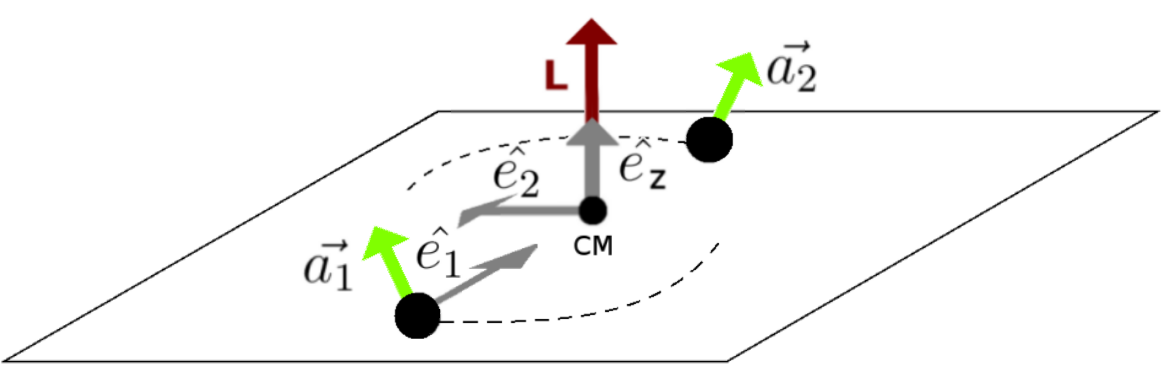
\includegraphics[width=0.7\textwidth]
{./figures/BinarySystem.png}
\caption{\small{Reference system that is used to apply the recoil velocity of the BH remnant.}}

\label{fig:RecoilReferenceSystem}
\end{figure}
%.........................................................................

We also correct for the eccentricity of the orbit using the formula proposed by \citep{Sopuerta2007}:

\eq{CorrectionEcc}
{ \vec{v}_{e} = \vec{v}_{\mbox{\tiny{ align, kick }}}( 1+e ) }

This approach is the most general one and will be implemented in our study.


%--------------------------------------------------------------------------------------------------
\subsection{Numerical implementation}
%--------------------------------------------------------------------------------------------------

In order to adapt the previous scheme to our simulations, we adopt a series of assumptions that 
facilitates the numerical implementation, namely:

\begin{itemize}
 \item Only merger events involving two BHs take place in the simulation. Three-BHs merger events
 are split up in two two-BHs mergers.
 \item The two BHs will merge once they are closer than the minimum of the softening lengths used to 
 compute the gas density for each BH.
 \item They will merge irrespectevely of their approach velocity. Usually, a criterion based on the
 local speed of sound would provide a more realistic scenario, however, as a first-order estimative,
 we do not apply this.
 \item The reference system used in the estimation of the kick velocity is built based on the
 state of the system just before the numerical coalescence. This clearly differs from the physical 
 coalescence as the binary system should take some time before the merger event, which happens after 
 the distance becomes less than smoothing length. However, this scale is by no means, well-resolved 
 in our simulations, so we neglect this time. We also assume that the angular momentum is not 
 significantly changed during the coalescence phase and the orbital plane, which defines our recoil 
 system, can be taken as the same in the numerical coalescence.
 \item Spin evolution is not considered here (at the moment). We assume that BHs accrete mass in a 
 chaotic and episodic way, as proposed by \citet{King2008}. This accretion mode regularize the spin
 of the BH as the infalling matter does not contribute constructively to spin up the BH. The random 
 and chaotic nature of the accretion makes the spin quickly converge to a value of $a = 0.3 \pm 0.2$.
\end{itemize}


\subsubsection{Setting up the spins}

Merger events are the only processes that can significantly spin up a BH, however the spin of the 
remnant should be quickly slowed down by chaotic and episodic gas accretion in a presumably short 
time scale, thereby erasing any ́"memory" of the initial conditions or the last merger \citep{King2008}. 
Instead of following spin evolution, we set up a random oriented spin for each BH prior to a merger.
The magnitude of the spin parameter is generated based on a normal distribution with $\bar{a} = 0.3$ 
and $2\sigma = 0.2$.

%.........................................................................
%Spin distribution
\begin{figure}[htbp]
\centering
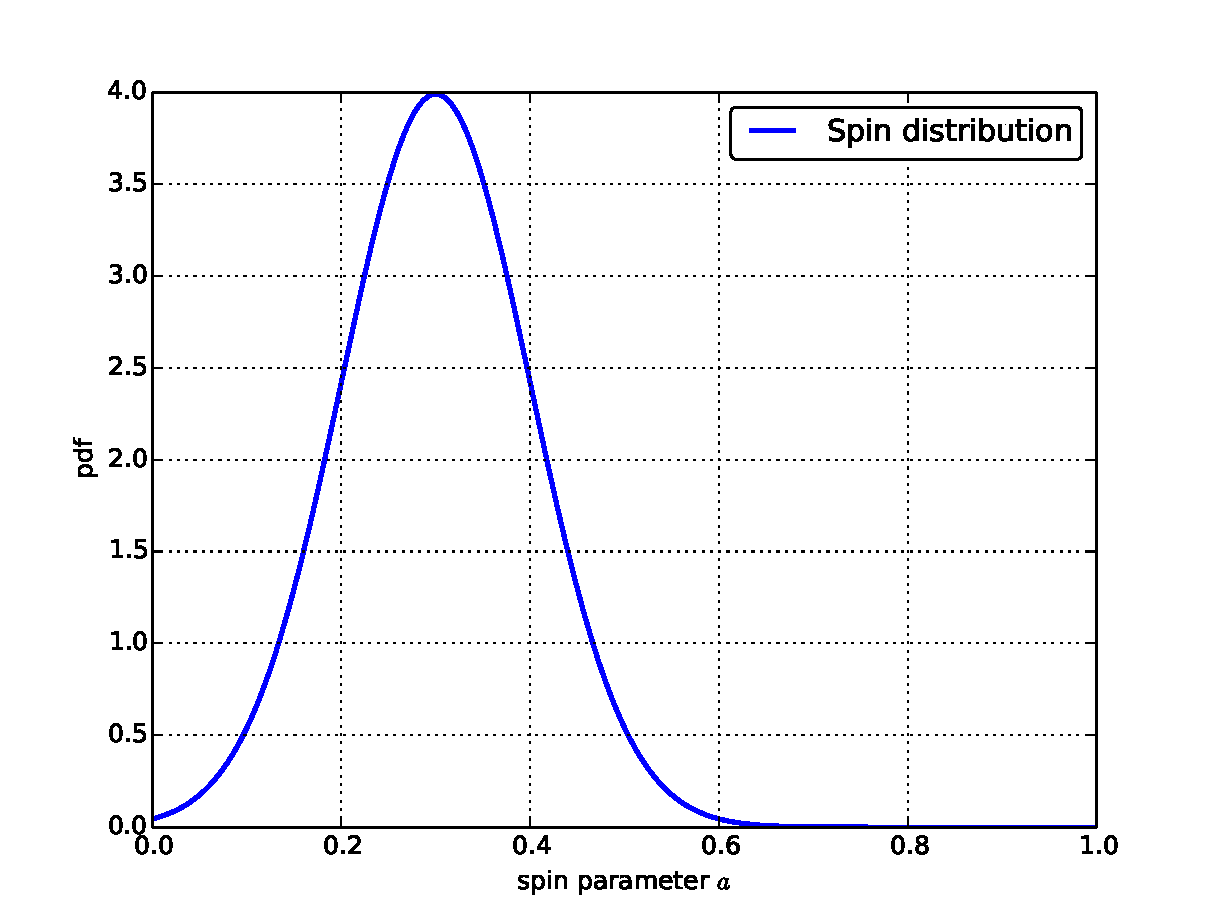
\includegraphics[width=0.50\textwidth]
{./figures/SpinDistribution.pdf}
\caption{\small{Spin distribution function to generate initial values prior to a merger.}}

\label{fig:SpinDistribution}
\end{figure}
%.........................................................................

\subsubsection{Defining reference system}

Prior to the merger, we have the next information from the two involved BHs: $m_1$, $\vec{r_1}$, 
$\vec{v_1}$, $m_2$, $\vec{r_2}$, $\vec{v_2}$ along with the two randomly generated spins $\vec{a_1}$
and $\vec{a_2}$. From this information, we proceed to construct the reference system where the recoil
merger kick will be referred. The respective two-body variables are then $\vec{r} = \vec{r_1} - 
\vec{r_2}$ and $\vec{v} = \vec{v_1} - \vec{v_2}$. The angular momentum of the binary is $\vec{L} = 
\vec{r}\times\vec{v}$. We define the orthonormal system $\hat{e_1}$, $\hat{e_2}$, $\hat{e_z}$ as 
$\hat{e_1} = \vec{r}/r$, $\hat{e_z} = \vec{L}/L$ and $\hat{e_2} = \hat{e_z}\times\hat{e_1}$

%==================================================================================================
\newpage
\bibliographystyle{latex/mn2e}
\renewcommand{\bibname}{8\ \ \ \ Bibliography}
\small
\bibliography{references.bib}
%==================================================================================================



\end{document}
